\emph{Neural networks} are a kind of machine learning model that is capable of detecting complex patterns in data. They consist of several \emph{layers} of connected \emph{neurons} that map input floating-point vectors to output vectors. \autoref{fig:2_basics/1_neural_networks/nn} shows an example of a neural network consisting of an input layer and two neural layers, also called \emph{linear layers}. The network forwards the input values on the left through the layers to produce the output values on the right.

\begin{figure}[t]
    \centering
    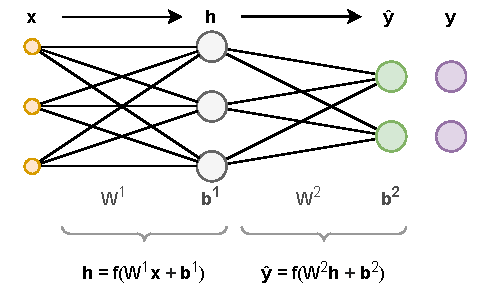
\includegraphics{2_basics/1_neural_networks/nn}
    \caption{Simple neural network consisting of the input layer, one hidden layer, and the output layer. The network's $i$th neural layer can be implemented by multiplying the layer's weight matrix $W^i$ with the layer input, adding the bias vector $b^i$, and applying the non-linear activation function $f$. By forwarding the network input $x$ through all layers, the network's predicted output $\hat{y}$ should approximate the ground truth output $y$.}
    \label{fig:2_basics/1_neural_networks/nn}
\end{figure}

The values of each layer's output neurons are calculated as weighted sums of the input values. Subsequently, a constant \emph{bias} is added and a non-linear \emph{activation function} is applied. Graphically, the weights can be represented as edges between the input and output neurons, while the bias values are assigned to the output neurons. Mathematically, the function of a linear layer can be calculated using matrix multiplication. For a neural layer that maps a $d$-dimensional input vector to an $e$-dimensional output vector, the layer's weights can be represented by a $d \times e$ \emph{weight matrix}. The layer's output vector can then be calculated by multiplying the input vector with the weight matrix, adding the $e$-dimensional bias vector, and applying the activation function.

By combining linear layers, complex models can be created that vary by the number of layers, the number of neurons, and the way neurons are connected. During the last decade, exponentially increasing data and processing power made \emph{deep networks} possible that consist of many layers and have the advantage that they can work without sophistically encoded input data because they come up with an encoding themselves. Other architecture concepts include \emph{recurrent} neural networks (RNNs), which repeat certain layers multiple times, and \emph{convolutional} neural networks (CNNs), which use filters to focus on local, close-by neurons. The semantics of the output layer depends on the network's intended task. An image \emph{classifier}, for example, yields probabilities that specify what output class the input most probably belongs to, while a \emph{natural language processing (NLP)} model might produce an abstract encoding of an input text.

To enable processing of the input data according to the desired output semantics, the \emph{parameters} of the network, in particular the edge weights and bias vectors, need to have appropriate values. Which exact values are appropriate depends on the kind of input data, the network architecture, and the intended outputs. The optimal parameters are determined by \emph{training} the model. During training, the network is repeatedly asked to make predictions for input data, which are then compared to the intended output data, the so-called \emph{ground truth}. In each step, the model's parameters are updated a bit to close the gap between predictions and ground truth. Technically, the \emph{backpropagation} algorithm is used to calculate the gradient of a \emph{loss function} that quantifies the deviation of the prediction from ground truth and applies that gradient to the model's parameters layer by layer, starting with the output layer, thus backpropagating the change through the network. Formally, the models parameters $\theta$ at step $t+1$ are calculated as described in \autoref{eq:2_basics/1_neural_networks/backprop}. The gradient of the loss function $L$ is multiplied by a \emph{learning rate} $\lambda$ and subtracted from the old parameter value.

\begin{align}
    \theta^{t+1} = \theta^t - \lambda \frac{\partial L(y, \hat{y})}{\partial \theta}
    \label{eq:2_basics/1_neural_networks/backprop}
\end{align}

In practice, the so-called \emph{optimizer} is responsible for calculating the parameter deltas from the gradient and applying them. The choice of the learning rate has a great influence on training: If the learning rate is too low, training takes too long, but if it is too high, the parameters may be updated too much and cannot settle at their optimum. Furthermore, local minima and plateaus in the loss function make it hard to reach the parameters that minimize the loss function the most. Advanced optimizers therefore resort to techniques like momentum, where the previous learning progress is taken into account, or changing the learning rate over time to reach optimal parameters in a reasonable time. Furthermore, the choice of the loss function also has a significant influence on learning success. The simple \emph{mean squared error (MSE)} loss do work, but advanced loss functions such as the \emph{binary cross-entropy (BCE)} loss used for binary classification accelerate training significantly. \autoref{eq:2_basics/1_neural_networks/mse} and~\ref{eq:2_basics/1_neural_networks/bce} compare the calculation of the MSE and BCE loss for a classifier with $n$ binary output classes.

\begin{align}
    L_{MSE}(y, \hat{y}) &= \frac{1}{n} \sum_{i=1}^n (y_i - \hat{y}_i)^2
    \label{eq:2_basics/1_neural_networks/mse} \\
    L_{BCE}(y, \hat{y}) &= \frac{1}{n} \sum_{i=1}^n y_i \cdot log( \hat{y}_i) + (1-y_i) \cdot log(1 - \hat{y}_i)
    \label{eq:2_basics/1_neural_networks/bce}
\end{align}

Besides selecting the appropriate learning rate, optimizer, and loss function, it is important to avoid \emph{overfitting} during training. This occurs when the model is trained for too long and the parameters are perfectly matched to the data used for training, but no longer work well on new data -- in that case, the model has learned the data by heart, so to speak. To prevent overfitting and identify the optimal time to stop training, the model is trained and validated on separate subsets of the dataset. During training on the \emph{training data}, it is regularly checked how the model behaves on the unseen \emph{validation data}, whose loss eventually reaches a minimum and increases again, which serves as a sign to terminate training. In addition to training and validation data, a portion of the data, the \emph{test data}, is kept under lock until the final \emph{evaluation} of the model. The reason for this is that researchers use the validation results to optimize the model, in a sense hand-tailoring it to the validation data. Therefore, the test data may be evaluated only after all the optimizations of the model have been completed to provide an objective measure of generalization to unseen data.

As mentioned before, neural networks proved successful in various domains, including NLP. Processing natural language opens many possibilities, for example, seamless human-machine interaction and knowledge extraction. What all NLP approaches have in common, is that they have to represent text in a way that makes it easy to process. The classical way to numericalize a text is using a \emph{bag of words}, which is a large vector whose elements represent words of a vocabulary. A concrete text is then encoded by setting all those elements to 1 that represent words occurring in the sentence. Although, the order of words is not preserved that way, bag of words have been used successfully with different machine learning models. A classical example would be a spam filter, implemented as a Bayesian network.

During the last decade, however, neural networks have had a breakthrough in NLP, because they solve a big problem of existing text encodings: Bag-of-words bear the problem that they are very \emph{sparse}, i.e. most of their entries are 0. Meanwhile, manually engineered feature vectors that target this problem are not only time-consuming to create but often tailored for specific data. Since then, deep networks have arisen and offer the ability to learn feature representations on their own - given enough time and training data. Due to the exponential growth in processing power and data, both constraints have been overcome, so that most state-of-the-art NLP models represent text using low-dimensional vectors, called \emph{embeddings}, today. They are called embeddings because the low-dimensional vector space the words are projected into is very dense compared to previous sparse encodings, so one can imagine how words have to be embedded into such an \emph{embedding space}. Thereby, the typical dimensionality of a word embedding space lies between 50 and 300.

Another breakthrough has been achieved in 2017 when \emph{transformers} outperformed other language models by far. Transformers focus on those parts of the input data that are particularly important for current processing, the concept of which is referred to as \emph{attention} because the transformer attends to certain words in its input text. Recently, attention has also been used in other domains, such as video processing~\cite{Bertasius2021IsSA}. One drawback of transformers is their sheer size. For example, recently, Google has trained the first transformer with over a trillion parameters~\cite{Fedus2021SwitchTS} on the Colossal Clean Crawled Corpus - a text dataset of 800GB in size in its default English version and of 26TB size in its multi-lingual version~\cite{C4}. As training such large models takes very long, even when using specialized processors, researchers provide \emph{pre-trained} word embeddings that were obtained from training a large model on a general-purpose task, such as predicting missing words in gap texts, using common text data. Users can then take these pre-trained embeddings as a basis and \emph{fine-tune} them regarding their specialized \emph{downstream task}.
